\todo{add introduction of subject and research area}



% As is discussed in section \ref{sec:processmining}, there exist many approaches for analysing process performance, but there are no approaches which specifically focus on resources. \todo{Move process mining chapter}

\section{Business Process Management}
Business Process Management (BPM) evolved from Workflow Management (WfMS) which originates from the 1990s \cite{hofstede2009modern,aalst2016business}. WfM and the corresponding Workflow Management Systems (WfMS) enabled organizations to decouple the control-flow perspective from application logic and business rules by making it possible to dynamically define workflow processes. WfMS focus primarily on process automation and many software vendors integrated a set of WfMS functionality into their software applications. The offered functionality per software vendor differed notably because of a lack an accepted standard \cite{dumas2013fundamentals, hofstede2009modern}.

Starting from the 2000s, Business Process Management (BPM) emerged from WfM and can be seen as an extension of WfM \cite{dumas2013fundamentals,aalst2016business}. BPM has a broader scope than WfM by focussing on process automation, as well on process management and the organization of BPM itself. With BPM, Business Process Management Systems (BPMS) arose, which enabled organizations to manage, control, and support their operational processes \cite{dumas2013fundamentals}. Furthermore, BPMS focus more on human factors and management support than WfM \cite{hofstede2009modern}. Additionally, because BPM is much broader than WfM, software is developed with specifically only at BPM functionality, namely: BPMS. BPMS handle all process management functionality and orchestrate a set of domain-specific applications. Therefore, BPMS can be seen as a central point in an organization which acts as a wrapper around all applications. \cite{dumas2013fundamentals}

The essential concept of BPMS is that they separate the control-flow, resource and application perspective \cite{hofstede2009modern}. The section each describe one of the perspectives.  

\subsection{Control-flow perspective}
The control-flow perspective of BPMS consists of process definitions which are independent of the application code. These process definitions are often in the form of a (graphical) process model, whereas there exist many different process modelling notations to model the processes. Examples of formal process modelling language are Petri Nets \cite{petrinets} and YAWL \cite{hofstede2009modern, yawl}, while a more commercially oriented modelling notation is Business Process Management Notation 2.0 (BPMN2) \cite{bpmn2}. Figure \ref{fig:bpmn} shows an example process modelled using BPMN2, where each process instance starts at the \textit{purchase order received} node, and flows to the right. 

\begin{figure}[h]
	\centering
    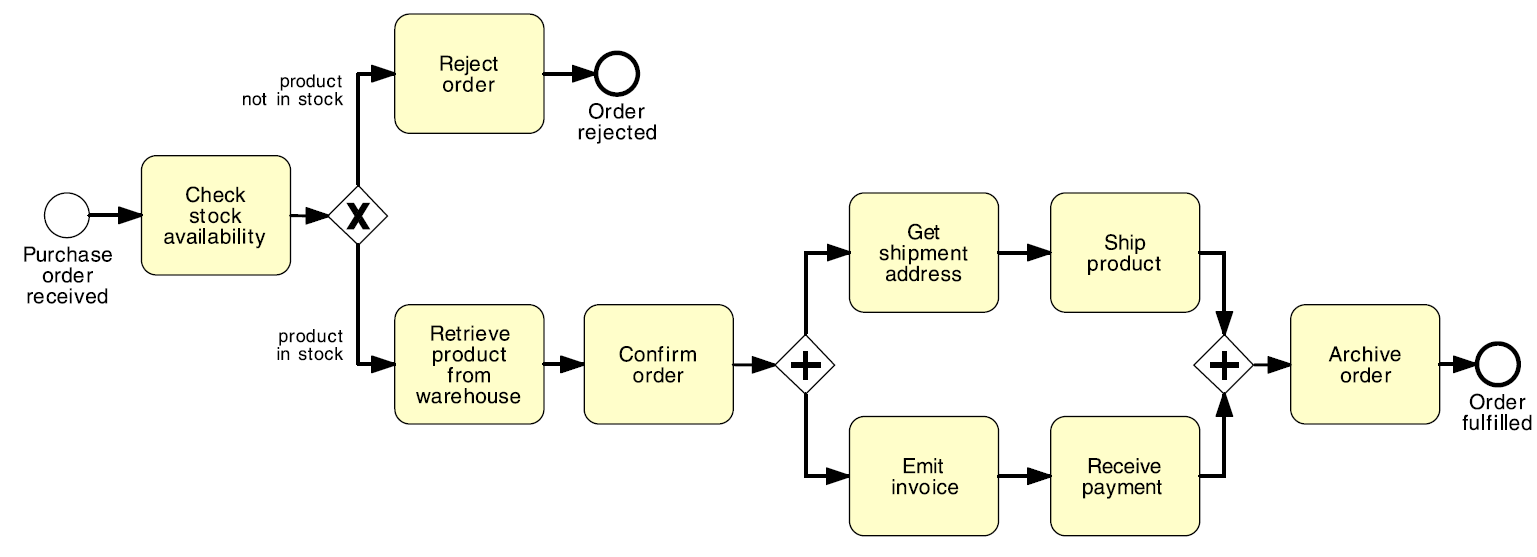
\includegraphics[width=\textwidth]{figures/bpmn.png}
    \caption[An example order fulfilment process in the Business Process Management Notation 2.0 ]{An example order fulfilment process in the Business Process Management Notation 2.0 {\cite{dumas2013fundamentals}} }
    \label{fig:bpmn}
\end{figure} 

% @article{dumas2013,
%   title={Fundamentals of business process management},
%   author={Dumas, Marlon},
%   year={2013}
% }

BPMS can interpret these process models and contains all kinds of functionality to deploy the described functionality of the process models in practice. For example, it can invoke financial systems to check whether the order is paid, notify users to pick certain items, communicate with customers and reorder new products. All this functionality is described in process models.

\subsection{Resource perspective} \label{section:introduction_resource_perspective}
The resource perspective consists of methods to manage the resources involved in the process executions. Resources can be either durable or non-durable. This thesis focusses on durable resources, i.e. resources that are claimed and released during the execution but are neither created nor destroyed before or after usage \cite{Huang2012,Huang2011a,Russell2004}. Examples of durable resources are employees, machines, books and cars. Examples of non-durable resources are software instances, raw materials and fuel.

Resources are the ones who perform the actual non-automated tasks and are therefore essential for the process execution. However, resources are not always available so the BPMS should plan the tasks according to a schedule. Furthermore, it is common that not all resources can perform all activities, thus the BPMS should also take this into account. Moreover, it is rather wasteful to randomly assign tasks to resources when a certain resource is already working on a large number of tasks, while the other resource has nothing to do. Finally, resources should also prioritize their tasks, because some tasks can have a higher priority than others and the resources only have a limited amount of time to perform a number of tasks. In order to take into account all these (and many more) problems, BPMS contain Work-allocation rules. The following sections discuss three types of resource work-allocation rules, namely: roles, resource allocation and resource prioritization.

\subsubsection{Roles}
Roles are part of Role-based access control (RBAC), which is a security policy dating back from 1996 \cite{rbac}. Today many organizations use RBAC to manage permissions within their organization \cite{rbac2,rbac}. In RBAC, each user has one or more role, whereas each role permits the access to one or more objects \cite{rbac2,rbac}. There are different kinds of permissions (e.g. read, write, own) and different kinds of objects (e.g. pictures, documents, databases) but for the scope of this paper, we only consider the permission to perform a certain activity. Whenever a user changes its position in the organization, its roles are changed. Similarly, whenever all users of a role (e.g. accountants) need permission to a new object, the role is simply changed. This is a major advantage over older security policies such as Discretionary Access Control (DAC) \cite{dac} and Mandatory Access Control (MAC) \cite{mac} where all permissions are stored on the user level so that for each user changes have to be made. 

Roles can be seen as a high-level work-allocation pattern in the context of BPM because it can determine which set of resources is allowed to perform a certain task. This narrows the search down for finding a resource to perform a certain task from the entire resource population to a set of resources. The next section describes how to further narrow down the search to an individual resource.

\subsubsection{Resource allocation}
Resource allocation rules or patterns define how to choose which resource should perform a certain task. There are two basic resource allocation pattern categories, namely: pull and push patterns \cite{hofstede2009modern, aalst2003workflow}. Pull patterns describe a situation where resources can decide which task they would like to execute and allocate the tasks to themselves. Contrary, push patterns describe a situation where the BPMS decides which resource should perform which tasks. Push patterns are much more complicated to implement because the pull patterns simply outsource the allocation to users whereas for push patterns the BPMS should perform the allocation automatically. Therefore, there are several elements of push patterns which each can help finding the most suitable resource for a given task as is discussed below. 

An important resource attribute is its availability, i.e. is the resource available? If so, what is its capacity? Is its capacity shared among other processes? How long is a resource available? The BPMS should, of course, only allocate tasks to resources which are available or becoming available in the near future, to prevent the situation that process instances keep waiting for resources which are simply not available. 

Another resource attribute is its preference or speciality, which describes what kind of tasks a resource prefers or is specialized in. This is important because specialized resources can better (e.g. higher quality/faster) perform certain activities than other resources. It can be the case that certain resources have more experience with handling certain tasks or simply like certain activities more. Note that a resource can also prefer certain case types (e.g. house loan request vs boat loan request or high-value loans vs low-value loans) instead of simply only certain activities.

Furthermore, another important resource attribute is its workload, i.e. the amount of  work allocated to a resource has. The workload should, of course, take into account the availability, but also the estimated task duration. The workload can be seen as a queue, where the tasks are waiting before the resource is available to perform the tasks. How resources handle such a queue is described in the next section. 

Finally, for compliance reasons, it might be the case that a previous resource allocation might limit the choice of resources in the future. For example, the 'four-eye' principle or 'dynamic separation of duty' pattern \cite{rbac} describes a situation where a resource might not be allowed to perform a task when it already performed another task for the same case. The four-eye principle can be used to prevent fraud. An example for such a situation is that a resource should not be able to create a large offer and also review the same offer because this offer should be reviewed by one of its peers. 

There are many attempts to combine the mentioned attributes into an optimal resource allocation model as is discussed in chapter \ref{chapter:background}. A rather naive method would be \textit{random allocation} or \textit{round robin} which both aim to provide each resource with an equal amount of tasks. An improvement could be to only look at workload, and allocate a task to the least-busiest resource, but this model still does not take into account availability and preference and will not motivate resources to finish their tasks as quickly as possible. 

\subsubsection{Resource Prioritization Rules}
Resource prioritization concerns only work list of a single resource and thus is relevant after tasks are allocated to a resource. The resource prioritization patterns describe how resources should handle the planning of its allocated tasks. There are various well-known resource prioritization policies, such as First-in-First-out (FiFo) and Last-in-Last-out (LiFo) \cite{hofstede2009modern}. Figure \ref{fig:fifolifo} illustrates FiFo and LiFo and shows that order of arrival is similar the execution order for FiFo. This is not the case for LiFo, where the latest arrived task is first performed. 

\begin{figure}[h]
	\centering
    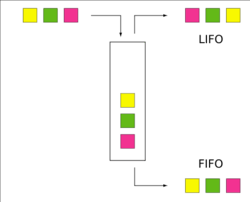
\includegraphics[]{figures/filo-lifo.png}
    \caption{A schematic illustration of FiFo and LiFo scheduling. The order of arrival is encoded into the worklist colours.}
    \label{fig:fifolifo}
\end{figure} 

\todo{Create better picture}

Furthermore, there are slightly more advanced policies such as Shortest Task in Queue and Shortest remaining case time. The Shortest Task in Queue prioritization policy simply estimates the duration of each event (e.g. by historical data or by heuristics) and the shortest task is chosen. The shortest remaining case policy estimates how long cases of the tasks in the worklist still need before they are finished, and picks the task with the shortest remaining case time. The latter policy aims to first finish all open cases before new cases are started. 

Finally, it is possible to extend each policy with priority, i.e. a different prioritization for high/low priority tasks. Each policy has its advantages and disadvantages and policies are seldom strictly followed. Each resource, role and department can have different prioritization rules.

\subsection{Application perspective}
The application perspective consists of a set of interoperability patterns which help the BPMS to communicate with external applications. The BPMS itself does not contain all functionality in an organization, it merely manages the process execution. This means that the BPMS is depended on many external applications. The BPMS can require external systems for the storage and retrieval of data (e.g. Customer Relationship Management (CRM) system for client data), but also outsource task execution to other systems (e.g. pay order task to the Enterprise Resource Planning (ERP) application) and can even be triggered by external systems (e.g. customer service desk received a call from a customer). Furthermore, communication can be synchronise and synchronize, and data routing can be dependent on various variables. There are also various methods for storing data such as repositories, relational databases, document-based databases and graph databases. 

The complete description of all these patterns is out-of-scope for this thesis. For more information, the reader is referred to \cite{russell2016workflow}.


\section{Process Mining} \label{sec:processmining}
Process Mining can be described as a set of quantitative analysis methods for business processes \cite{aalst2016process}. It is therefore often associated with the Business Process Management (BPM) domain \cite{aalst2013business} because of the focus on business processes, and the Data Mining domain \cite{kaufinann2006data} because of the focus on data and quantitative analysis methods. Process Mining is an emerging research field and gains many attention from the corporate and (semi-)governmental sectors \cite{aalst2011process,aalst2016process,aalst2012process}.

The basis of process mining is an Event Log \cite{aalst2016process}, which can be described as a dataset containing process related data. An Event Log contains at least a set of events, whereas each event describes change in time. Events have a time of occurrence, the type of task (activity) which is executed and the user who performed the event. Furthermore, the events are grouped in cases, whereas each case is a logical categorization of events, for example: each case describes a customer complaint handling, bank loan request or permit request. An Event log contains arbitrary many cases and each case can contain arbitrary many events.  

The three traditional pillars of process mining are: \textit{process discovery}, \textit{conformance checking} and \textit{process enhancement} and are all actively researched \cite{aalst2016process,aalst2011process}. \textit{Process discovery} focusses on describing the event log in terms of a process model. It aims to find the best possible process model for a given event log. \textit{Conformance checking} focusses on finding deviations of an event log to certain policies and is therefore mainly of interests for auditing purposes. Finally, \textit{process enhancement} aims to improve a discovered process model based on an event log by enriching the process model with additional or higher quality information.  

Furthermore, process mining has different perspectives \cite{aalst2016process}. Traditionally, the most important perspective is the \textit{control-flow} perspective, which describes the logical relations between activities and is often visualized in the form of a process model and is an integral part of the process discovery pillar \cite{discovery}. Another perspective which is often analysed is the \textit{case} perspective, which contains a collection of all events for each case. Furthermore, the \textit{organizational} perspective is also researched and aims to provide insights in the organizational hierarchy and rules such as identifying social networks \cite{van2007business,socialmining}. Moreover, the \textit{data} perspective contains additional optional data attributes and aims to find interesting correlations to improve process understanding or for the purpose of conformance checking \cite{DeLeoni2012,rogge2016log}. Finally, a well-studied BPM and process mining perspective is the \textit{time} or \textit{performance} perspective which describes the timing of events \cite{hornix2007performance,aalst2012replaying, aalst2009performancevis}. This perspective contains essential information for traditional business process improvements such as identifying bottlenecks and lowering throughput times.

One perspective which is missing and is often not considered explicitly is the \textit{resource} perspective \cite{Zhao2015}. The resource perspective contains information on which individual resource (e.g. employee, machine or system) performs which events. The resource perspective is somewhat related to the organizational and performance perspective. However, the former does not focus on individual resources and the latter tends to focus on the process as a whole and not on individual resources. This seems remarkable because resources seem to have a major impact on the process performance as they (i.e. employees) tend to be unpredictable, unreliable, error-prone and performing tasks with varying amounts of quality \cite{Pika2015}. Many BPM research acknowledges the fact that resources are an important factor, perhaps event one of the most important factors, of a business process \cite{baccarini2004management, Pika2015,thevendran2004perception}. 


\section{ProcessGold}
\todo{The introduction should contain a description of ProcessGold}


\section{Thesis description}
This section outlines the content of this thesis and is composed of a main research question and several supporting sub-research questions. The main research question is defined as:

\vspace{.5cm}
\textbf{RQ} How to analyse the impact of resources on cases and the impact of all cases on resources?
\newline


The question specifically focuses on the resource perspective. The resources perform the tasks of business processes and have therefore a significant impact on the process execution. Therefore, it is important to have a framework for analysing resources in a structured manner. The first step towards creating such a structured analyse method is to identify what is the current state-of-the-art in this area. The second step is to find relevant questions that need to be answered by the analysis method. Both steps are summarised in the first two sub-research questions, which are shown below. 

\begin{enumerate}
	\item[\textbf{RQ1}] What is the current state-of-the-art of resource-perspective analysis? 
    \item[\textbf{RQ2}] What are relevant resource-related questions and problems?
\end{enumerate}

\noindent
In order to answer RQ1, a literature study should be concocted to identify the latest developments in the resource-perspective analysis. Similarly, a literature study of the Business Process Management literature is also required in order to answer RQ2. Additionally, interviews with domain experts and consultants can also contribute to answering this research question. 

The structure of the rest of this document is as follows. Chapter \ref{chapter:background} aims to answer RQ1 by discussing the state-of-the-art literature on resource analysis. Chapter \ref{chapter:thesisoutline} then discusses relevant questions and problems for the resource perspective in order to answer RQ2. \todo{Add other chapters}



















